


En esta parte abarcaremos qué es un robot, la posible equivalencia entre robot y autómata y la evolución de estos conceptos a lo largo del tiempo. Es decir claro queda que un robot debe ser un tipo de máquina, pero la noción de lo que es una máquina ha variado significativamente a lo largo del tiempo. \\

Nadie dudaría sobre la veracidad de la siguiente afirmación 'Un ordenador es una máquina'; sin embargo, hay una diferencia cualitativa importante entre un ordenador y un actuador mecánico, por ejemplo: una puerta automática. \\

La noción de automatismo será clave para discernir qué es o no es un robot. \\

\subsection{ Sobre la noción de máquina}


Partimos del concepto más simple hasta ahora mencionado, 'la máquina' y de entre ellas las más sencillas de entender, las máquinas aristotélicas, siglo III A.C: \\

-Simple machine, any of several devices with few or no moving parts that are used to modify motion and force in order to perform work. (Enciclopedia Britannica) \\


Serían: El plano inclinado, La palanca, La polea, El torno, La cuña y el tornillo. El primer enfoque de qué es una máquina está mucho más relacionado con el equilibro de fuerzas en un sistema estático que con la abstracta definición de qué cosas son máquinas que tenemos hoy en día. 

Llegamos al siglo XVI, la idea de una máquina es la de un objeto que cuyas partes distinguibles pueden ser clasificadas como una de las anteriores máquinas simples. \\

- 'Thus Leonardo was the first to advocate the necessity of a science of mechanisms.' -  \\

- ' A book about the nature of mechanism must precede a book about their aplications' \\

Ladislao Retti: 'The Unknown Leonardo' \\

Este pensamiento hace avanzar la 'ciencia de la máquina' , en los siglos anteriores el estudio de las máquinas era empírico alejado de cualquier conceptualización teórica. Es decir, el conjunto de las máquinas estaba definido por extensión. Este paso cualitativo permitió el comienzo de la conceptualización teórica de las máquinas.

Vemos el auge de este pensamiento en el mecanicismo filosófico. Encontramos grandes matemáticos como Descartes o Newton participando en esta teoría. El concepto de máquina evoluciona, una máquina será aquel objeto descriptible mediante las leyes de la física, la mecánica (clásica) concretamente. Vemos una definición intensiva en contraposición al pensamiento anterior. Nace con Descartes el pensamiento de que una máquina no es necesariamente un objeto artificial, considerando los animales de manera mecánica, complicada, sí, pero máquina \textit{per se}. \\

La evolución del termino 'maquina' se va alejando cada vez más de la aplicación concreta de la 'maquina' en sí, hacia el concepto de que una máquina es aquel objeto cuyo comportamiento es determinista. \\

- A machine (or mechanical device) is a mechanical structure that uses power to apply forces and control movement to perform an intended action (Wikipedia) \\

A nuestros ojos, la definición parece incompleta por lo pronto, pues en el conjunto que define encontraríamos las máquinas simples,los coches pero no los ordenadores. ¿Es que acaso no son máquinas? Si bien es cierto que un ordenador puede comportarse de este modo, no es una cualidad intrínseca de un ordenador. Es decir: podemos conectar un actuador mecánico para que cumpla la definición, pero no tiene mucho sentido que al desconectárselo deje de ser una máquina. \\

El elemento invariante es su cualidad determinística, una máquina actúa conforme a un patrón. La categorización de un objeto físico como una máquina se produce cuando de su comportamiento se elimina el azar, se puede conocer su estado exacto después de recibir un estímulo.



\subsubsection{ ¿Qué es un autómata? (mecánica)}

Queda claro que un autómata debería ser algún tipo de máquina, es decir: en esencia debería presentar un comportamiento determinista. Aquí cobra importancia la noción de 'automatización'.

Autómata proviene de la palabra griega \textbf{\textgreek{αὐτόματος}} , cuya traducción seria '\textbf{que se mueve por si mismo}'. Es decir, la forma clásica de conceptualizar un autómata sería justo la de automatización, sería por tanto una máquina capaz de actuar sin intervención humana. Dejaríamos fuera de este conjunto a todas la máquinas simples y a los coches por ejemplo, pues no son capaces de llevar a cabo su función sin una intervencion expresa.




\subsection{ Conceptualización de la máquina y el autómata.}

Hemos hablado de lo complicado que resulta dar una definición completa de estos conceptos, pues aunque todos sepamos qué es una maquina por extensión, las cualidades que comparten los objetos que llamamos máquinas pueden llegar a ser muy excasas.

\subsubsection{ Algebras de Boole y sistemas combinacionales}

En el siglo XIX se da otro gran avance cualitativo sobre el entendimiento de qué cosas son máquinas, alejándonos de la definición "mecánica" de los mecanicistas y entrando en el campo de la lógica.

Las algebras de Boole son la base teórica de los sistemas combinacionales. Un sistema combinacional es una máquina (según hemos definido) cuya salida es únicamente función de su entrada, es decir, no presenta memoria sobre ningún estado pasado. Este será un aspecto fundamental en el avance de las "máquinas", su memoria, la cualidad de tener memoria sobre un uso anterior marcará toda una escala de complejidad.


La realización de este concepto se ve con gran claridad en los circuitos lógicos, a partir de operaciones simples ( como son la negación, la disyunción y la conjunción ) podemos llegar a expresar teóricamente cuál sería el funcionamiento de un sistema lo suficientemente complejo como para realizar operaciones artiméticas a mayor velocidad que un humano.

Queremos destacar que aunque estos sistemas se consideran típicamente como digitales, hechos a base de transistores recibiendo impulsos eléctricos, no tienen una diferencia cualitativa importante en cuanto a capacidad de computo o expresividad con un sistema mecánico clásico.

<!-- TODO  ejemplo de sist combinacional -->

%En 1642 el filósfo y matemático francés Blaise Pascal inventó una calculadora mecánica, *La pascalina*. Aunque es evidente que hay una gran diferencia entre una calculadora mecánica y una digital, ambas pueden conceptualizarse como sistemas combinacionales; ya que ninguna de las dos tiene, memoria sobre ejecuciones anteriores (estados) y el sistema, sean cuales sean sus actuadores, produce una salida como función única de una entrada. -->


\subsection{ Autómatas finitos}


En el siglo XX nace la teoría de autómatas como siguiente nivel de conceptualización sobre qué son las máquinas y qué pueden hacer, la pregunta fundamental de este momento histórico es : ¿Qué problemas puede resolver una máquina?.

Daremos ahora una definición de autómata alejada del mecanicismo anterior, más parecido al modelo abstracto de las algebras de Boole: Un autómata finito es una máquina (abstracta) cuya salida no depende solo de la entrada actual.

Un autómata finito tiene estados, posiciones de memoria que dependerán de las entradas anteriores, esto eleva la capacidad expresiva del autómata muy por encima de la del S.C. \\

- En electrónica un autómata es un sistema secuencial, aunque en ocasiones la palabra es utilizada también para referirse a un robot. [...] Sin embargo, la rápida evolución de los autómatas hace que esta definición no esté cerrada. (Wikipedia)- \\

Aquí un sistema secuencial es justo lo que hemos definido como autómata, un sistema combinacional dotado de memoria.  Un ejemplo muy sencillo de un cálculo que podría hacerse con un autómata finito y no bastaría con un sistema combinacional sería la tarea de decidir si un conjunto de ceros es par o impar. Esto puede parecer una tarea trivial pero es un cálculo recurrente en la comprobación de error.

<!-- Meter autómata -->

<!-- TODO: Ejemplo de primeros  autómatas -->

\subsubsection{Aumentando la abstracción: Lenguajes y problemas }


Esta evolución sobre lo que era una máquina y qué problemas podía resolver planteó el mismo porblema que habíamos subrayado antes. ¿Si podemos clasificar las máquinas que tenemos según su complejidad, podríamos hacerlo con los problemas?

Este es fundamentalmente el objeto de estudio de la teoría de autómatas, pues responde fundamentalmente a la pregunta: ¿ Qué máquina necesito para resolver este problema?

La definición del lenguaje formal como se hace en esta teoría es bastante natural:


Sea  $\mathcal{A}$ un conjunto finito de símbolos, a este conjunto lo llamaremos alfabeto, muy en consonancia con el uso popular del concepto. A los símbolos de $\mathcal{A}$ se les llamará letras, a las secuencias finitas de letras, palabras, y a todas las palabras que se puedan formar con las letras se las conoce como lenguaje generado por $\mathcal{A}$ o por sintetizar $\mathcal{A}^{*}$. Un lenguaje sobre $\mathcal{A}$, será un subconjunto de su lenguaje generado. Esto es:


$$ \mathcal{L} \text{ es un lenguaje sobre } \mathcal{A}  \iff \mathcal{L} \subset \mathcal{A^{*}} $$


Hasta aquí existe un paralelismo evidente con lo que asociaríamos con un lenguaje de manera popular. Pues bien, existe una relación entre las categorías de complejidad que mencionamos antes y los lenguajes. \\ \newpage

Por ejemplo, definamos el siguiente lenguaje, palabras sobre $\{0,1\}$ tales que tengan un número par de 0's.

\begin{equation}
\mathcal{L} = \{\omega \in \{0,1\}^{*} : \text{ $\omega$ tiene un nº par de 0's} \}
\end{equation}


\begin{center}
	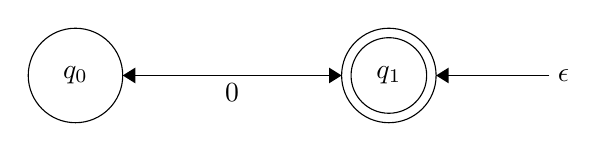
\begin{tikzpicture}[scale=0.2]
	\tikzstyle{every node}+=[inner sep=0pt]
	\draw [black] (40.6,-19.3) circle (3);
	\draw (40.6,-19.3) node {$q_1$};
	\draw [black] (40.6,-19.3) circle (2.4);
	\draw [black] (20.7,-19.3) circle (3);
	\draw (20.7,-19.3) node {$q_0$};
	\draw [black] (37.6,-19.3) -- (23.7,-19.3);
	\fill [black] (23.7,-19.3) -- (24.5,-19.8) -- (24.5,-18.8);
	\draw [black] (23.7,-19.3) -- (37.6,-19.3);
	\fill [black] (37.6,-19.3) -- (36.8,-18.8) -- (36.8,-19.8);
	\draw (30.65,-19.8) node [below] {$0$};
	\draw [black] (50.8,-19.3) -- (43.6,-19.3);
	\draw (51.3,-19.3) node [right] {$\epsilon$};
	\fill [black] (43.6,-19.3) -- (44.4,-19.8) -- (44.4,-18.8);
	\end{tikzpicture}
\end{center}

%TODO citar el libro que has sacado de la biblioteca

El siguiente autómata sería capaz de clasificar las palabras sobre el lenguaje generado por $\{0,1\}^{*}$ de manera que podría decirnos qué palabras pertenecen exactamente al lenguaje. La correspondencia entre lenguaje y autómata es aun mayor, porque de hecho, este autómata solo acepta las palabras del lenguaje $\mathcal{L}$. Una vez introducidos los conceptos daremos una definición rigurosa. \\

Un autómata se modela de la siguiente manera, es una tupla de 5 elementos: $(Q, \mathcal{A}, q_0, \delta, F)$

\begin{itemize}
	\item $Q$ : Conjunto finito de estados que numeramos $ q_0 \dots q_n$
	\item $\mathcal{A}$: Alfabeto, conjunto finito de símbolos sobre el que se crearán palabras del lenguaje.
	\item $q_0$ el estado inicial.
	\item $\delta :Q\times \mathcal{A} \rightarrow Q$. Función que nos indica como leer la palabra.
	\item $F$ : Conjunto de estados finales
\end{itemize}


Explicaremos ahora con detenimiento la relación entre los lenguajes y los autómatas pues son dos maneras de hablar del mismo concepto. Supongamos el siguiente lenguaje sobre $\{0,1\}$: Si la palabra empieza por 1 no pertenece al lenguaje, si empieza por 0 sí. El autómata que únicamente acepta las palabras de este lenguaje es el siguiente:

\begin{center}
	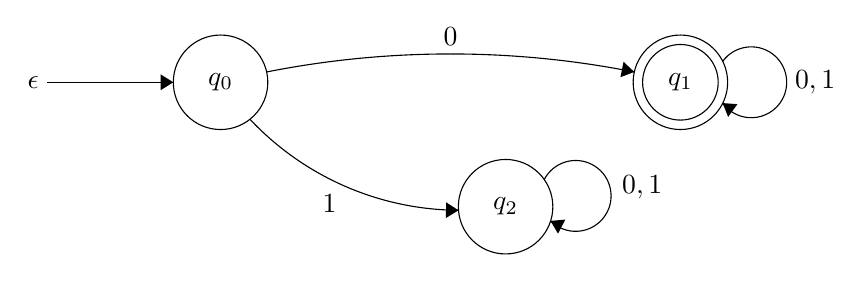
\begin{tikzpicture}[scale=0.2]
	\tikzstyle{every node}+=[inner sep=0pt]
	\draw [black] (20.6,-27.7) circle (3);
	\draw (20.6,-27.7) node {$q_0$};
	\draw [black] (49.8,-27.7) circle (3);
	\draw (49.8,-27.7) node {$q_1$};
	\draw [black] (49.8,-27.7) circle (2.4);
	\draw [black] (38.7,-35.6) circle (3);
	\draw (38.7,-35.6) node {$q_2$};
	\draw [black] (23.527,-27.044) arc (101.19936:78.80064:60.1);
	\fill [black] (46.87,-27.04) -- (46.19,-26.4) -- (45.99,-27.38);
	\draw (35.2,-25.4) node [above] {$0$};
	\draw [black] (52.48,-26.377) arc (144:-144:2.25);
	\draw (57.05,-27.7) node [right] {$0,1$};
	\fill [black] (52.48,-29.02) -- (52.83,-29.9) -- (53.42,-29.09);
	\draw [black] (35.712,-35.827) arc (-90.34893:-136.81015:18.322);
	\fill [black] (35.71,-35.83) -- (34.92,-35.32) -- (34.91,-36.32);
	\draw (27.52,-34.81) node [below] {$1$};
	\draw [black] (41.148,-33.885) arc (152.74451:-135.25549:2.25);
	\draw (46.07,-34.38) node [right] {$0,1$};
	\fill [black] (41.55,-36.5) -- (42.03,-37.31) -- (42.49,-36.42);
	\draw [black] (9.6,-27.7) -- (17.6,-27.7);
	\draw (9.1,-27.7) node [left] {$\epsilon$};
	\fill [black] (17.6,-27.7) -- (16.8,-27.2) -- (16.8,-28.2);
	\end{tikzpicture}
\end{center}



Un autómata puede presentarse también a modo de grafo como vemos, los estados se representan como nodos y los arcos representan las transiciones que modela al función $\delta(\cdot)$.Es decir, leemos la palabra de izquierda a derecha y por cada símbolo de la palabra, buscamos cuál es la transición asociada al estado en que nos encontramos y el símbolo que estamos leyendo.

Ahora bien, uno de los estados está marcado con dos circunferencias, este es un estado final, al ser el único: $F = \{q_1\}$. El resto de los elementos de la tupla serían:

\begin{multicols}{2}
	\begin{itemize}
		\item $Q =\{q_0,q_1,q_2\}$
		\item $\mathcal{A} = \{0,1\}$
		\item $F = \{q_1\}$
	\end{itemize}
	
\end{multicols}

En cuanto a la función de transición, tendremos que el par $(a,q_i)$ pertenece al dominio de la función, si en el grafo existe un arco que salga de $q_i$ con etiqueta $a$. Las transiciones serían las siguientes:

\begin{multicols}{2}
	\begin{itemize}
		\item $\delta(0,q_0)=q_1$
		\item $\delta(1,q_0)=q_2$
		\item $\delta(a,q_1)=q_1 \ \forall a \in \{0,1\}$
		\item $\delta(a,q_2)=q_2 \ \forall a \in \{0,1\}$
	\end{itemize}
\end{multicols}

El símbolo $\epsilon$ se reserva para la palabra vacía, que es una entelequia que simboliza la palabra que no contiene ninguna letra.





\subsubsection{No-Determinismo}

Los autómatas que hemos examinado antes son deterministas, es decir, dada una entrada y partiendo de un estado, es trivial averiguar en qué estado acabaremos una vez leída. Sin embargo podemos considerar qué pasaría si nuestra función define las siguientes transiciones:

\begin{multicols}{2}
	\begin{itemize}
		\item $\delta(0,q_i)=q_j$
		\item $\delta(0,q_i)=q_k \hspace{2cm} j\neq k$
	\end{itemize}
\end{multicols}


Es decir: ¿Qué hacemos si estando el estado $q_i$ leemos un $0$? ¿Nos vamos a $q_j$ o a $q_k$? La respuesta no es simple. Los autómatas finitos no deterministas nacen por su enorme capacidad de expresión y su definición menos rigurosa que la de los anteriores. Sería una gran ventaja que fuesen equivalente, de manera que pudiésemos usar este último, más sencillo de definir, y aun así tener la potencia expresiva del anterior. La respuesta será que sí. \\


Su definición es parecida a la anterior salvo por un detalle, la función de transición:

$$\delta :Q\times \mathcal{A} \rightarrow \mathcal{P}(Q)$$

Aquí $\mathcal{P}(Q)$ es el conjunto potencia de $Q$, las partes de $Q$, es decir, dado un estado y un símbolo, podemos construir un autómata que tenga una arco conectando este estado $q_i$ con todos los demás incluyendo el mismo.


Supongamos el siguiente problema, queremos crear un autómata que nos distinga  si una palabra pertenece a este lenguaje:

$$\{ \omega \in \{0,1\}^* : \omega \text{ tiene un número par de 0's} \} \cup \{\omega  \in \{0,1\}^*: \omega \text{ contiene al cadena }  101 \}$$

\begin{center}
	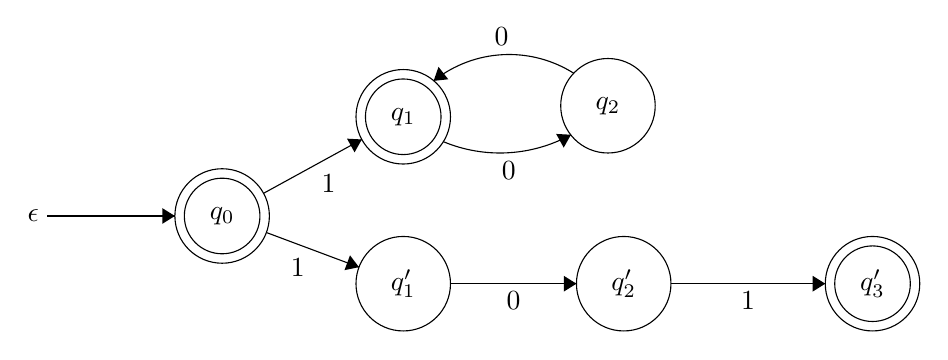
\begin{tikzpicture}[scale=0.2]
	\tikzstyle{every node}+=[inner sep=0pt]
	\draw [black] (17.2,-29) circle (3);
	\draw (17.2,-29) node {$q_0$};
	\draw [black] (17.2,-29) circle (2.4);
	\draw [black] (28.7,-22.7) circle (3);
	\draw (28.7,-22.7) node {$q_1$};
	\draw [black] (28.7,-22.7) circle (2.4);
	\draw [black] (28.7,-33.3) circle (3);
	\draw (28.7,-33.3) node {$q_1'$};
	\draw [black] (41.7,-22) circle (3);
	\draw (41.7,-22) node {$q_2$};
	\draw [black] (42.7,-33.3) circle (3);
	\draw (42.7,-33.3) node {$q_2'$};
	\draw [black] (58.5,-33.3) circle (3);
	\draw (58.5,-33.3) node {$q_3'$};
	\draw [black] (58.5,-33.3) circle (2.4);
	\draw [black] (6.1,-29) -- (14.2,-29);
	\draw (5.6,-29) node [left] {$\epsilon$};
	\fill [black] (14.2,-29) -- (13.4,-28.5) -- (13.4,-29.5);
	\draw [black] (19.83,-27.56) -- (26.07,-24.14);
	\fill [black] (26.07,-24.14) -- (25.13,-24.09) -- (25.61,-24.96);
	\draw (23.95,-26.35) node [below] {$1$};
	\draw [black] (20.01,-30.05) -- (25.89,-32.25);
	\fill [black] (25.89,-32.25) -- (25.32,-31.5) -- (24.97,-32.44);
	\draw (22.01,-31.67) node [below] {$1$};
	\draw [black] (39.348,-23.841) arc (-61.15181:-112.68383:9.343);
	\fill [black] (39.35,-23.84) -- (38.41,-23.79) -- (38.89,-24.66);
	\draw (35.4,-25.54) node [below] {$0$};
	\draw [black] (31.7,-33.3) -- (39.7,-33.3);
	\fill [black] (39.7,-33.3) -- (38.9,-32.8) -- (38.9,-33.8);
	\draw (35.7,-33.8) node [below] {$0$};
	\draw [black] (45.7,-33.3) -- (55.5,-33.3);
	\fill [black] (55.5,-33.3) -- (54.7,-32.8) -- (54.7,-33.8);
	\draw (50.6,-33.8) node [below] {$1$};
	\draw [black] (30.625,-20.424) arc (128.5933:57.57106:7.686);
	\fill [black] (30.63,-20.42) -- (31.56,-20.32) -- (30.94,-19.53);
	\draw (34.95,-18.21) node [above] {$0$};
	\end{tikzpicture}
\end{center}

Si nos fijamos, los estados $q_i'$ y los $q_i'$ conforman 2 autómatas independientes, que hemos unido usando el no-determinismo en la transición $\delta(q_0,1)$ hemos dado un autómata que reconoce únicamente las palabras del lenguaje unión, uniendo los autómatas.

Esto se puede extender todavía más, introduciendo el concepto de las transiciones nulas. Una transición nula es la manera más cómoda de unir dos autómatas pues puedes moverte por libertad por todos los estados entre los que haya una transición nula. Intuitivamente esto quiere decir que podemos ir de un estado a otro sin leer el símbolo actual. 


\subsubsection{Ejemplos de Autómatas}

Después de estas consideraciones queda pensar,cuál es el papel de estos modelos en cuanto a su papel en temas de robótica. Pues pensemos en una función relativamente simple que querríamos que tuviese un robot, la comunicación por ejemplo.

Un protocolo de comunicación es de los requerimientos más fundamentales ya no en la robótica sino en cualquier sistema de relativa complejidad pues la función en sí es tan importante como la existencia de una interfaz de comunicación con el usuario. No nos referimos necesariamente a la capacidad de expresión del agente, sino a la existencia de un protocolo que le permita transmitir información de forma coherente y exacta con el humano con el que interaccione, aunque sea este su programador.

Hablamos por ejemplo, da la implementación del protocolo TCP/IP, que en el fondo, es una máquina de estados finita o como lo venimos llamando, un autómata finito determinista. Daremos un ejemplo de cómo modelar un sistema de autentificación de usuarios con una máquina de estados muy simple.

\begin{itemize}
	\item $q_0$ Estado Inicial: En espera
	\item $F=\{q_1\}$ Único estado final : Autentificado
	\item $\mathcal{A}=\{001,010,011,000\}$
\end{itemize}

En cuanto a la función de transición. Supongamos que nuestro sistema incorpora la siguiente directivas:

\begin{multicols}{2}
	\begin{itemize}
		\item Envío de contraseña incorrecta: $001$
		\item Envío de contraseña correcta: $010$
		\item Salir: $011$
		\item Error: $000$
	\end{itemize}
\end{multicols}

\vspace{1cm}

\begin{center}
	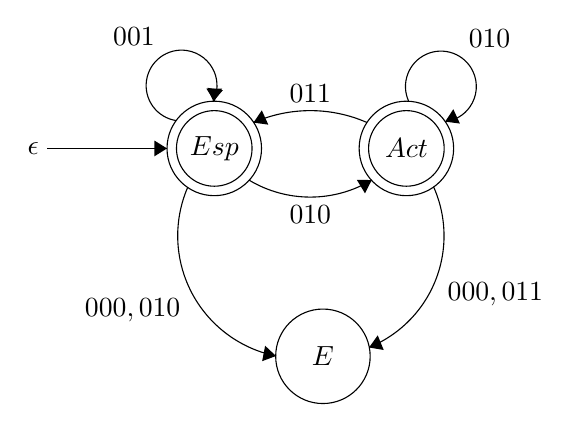
\begin{tikzpicture}[scale=0.2]
	\tikzstyle{every node}+=[inner sep=0pt]
	\draw [black] (37,-18.6) circle (3);
	\draw (37,-18.6) node {$Esp$};
	\draw [black] (37,-18.6) circle (2.4);
	\draw [black] (49.2,-18.6) circle (3);
	\draw (49.2,-18.6) node {$Act$};
	\draw [black] (49.2,-18.6) circle (2.4);
	\draw [black] (43.9,-31.8) circle (3);
	\draw (43.9,-31.8) node {$E$};
	\draw [black] (39.494,-16.958) arc (113.75402:66.24598:8.952);
	\fill [black] (39.49,-16.96) -- (40.43,-17.09) -- (40.02,-16.18);
	\draw (43.1,-15.7) node [above] {$011$};
	\draw [black] (46.998,-20.609) arc (-58.98762:-121.01238:7.566);
	\fill [black] (47,-20.61) -- (46.05,-20.59) -- (46.57,-21.45);
	\draw (43.1,-22.19) node [below] {$010$};
	\draw [black] (37,-15.5) -- (37,-15.6);
	\fill [black] (37,-15.6) -- (37.5,-14.8) -- (36.5,-14.8);
	\draw [black] (34.59,-16.833) arc (261.47443:-26.52557:2.25);
	\draw (31.9,-12.1) node [above] {$001$};
	\fill [black] (36.94,-15.61) -- (37.55,-14.9) -- (36.56,-14.75);
	\draw [black] (26.4,-18.6) -- (34,-18.6);
	\draw (25.9,-18.6) node [left] {$\epsilon$};
	\fill [black] (34,-18.6) -- (33.2,-18.1) -- (33.2,-19.1);
	\draw [black] (50.924,-21.032) arc (24.0977:-67.85012:7.646);
	\fill [black] (46.83,-31.24) -- (47.76,-31.4) -- (47.38,-30.47);
	\draw (51.79,-27.89) node [right] {${000,011}$};
	\draw [black] (40.919,-31.779) arc (-101.43921:-203.36619:7.786);
	\fill [black] (40.92,-31.78) -- (40.23,-31.13) -- (40.04,-32.11);
	\draw (34.88,-28.9) node [left] {${000,010}$};
	\draw [black] (49.35,-15.615) arc (204.86229:-83.13771:2.25);
	\draw (54.48,-12.2) node [above] {$010$};
	\fill [black] (51.66,-16.9) -- (52.6,-17.02) -- (52.18,-16.11);
	\end{tikzpicture}
\end{center}


Podríamos codificar los estados de $Esp$ (espera) y $Act$ (activo) como $000$ y $100$ con lo que tendríamos el estado de error ($E$) codificado como $101$. El autómata describe los posibles pasos en la autentificación de un usuario en un sistema, los estados de 'espera' y 'activo' serían finales dado que son estados 'correctos' en un posible sistema como este. El estado de error, describe justo eso, un comando que no se esperaba dado el estado de la comunicación en el que estábamos. Con este modelo podríamos construir un sistema de autentificación de usuarios usando 3 bits unicamente.


\subsection{La jerarquía de Chomsky}

El lenguaje que puede reconocer un autómata finito recibe el nombre de lenguaje regular, ya sea el autómata determinista, no-determinista o no-determinista con transiciones nulas, pues como comentábamos el paso de uno a otro se lleva a cabo mediante un procedimiento algorítmico. 

Un concepto íntimamente relacionado con el de lenguaje, como aquí lo hemos visto, es el concepto de gramática, a saber: las reglas de producción a seguir para crear una palabra del lenguaje. Distinguiremos símbolos terminales (escritos con letras mayúsculas) y símbolos terminales, notados con letras minúsculas. La gramática asociada a un lenguaje regular tiene la siguiente forma:


$$ A \rightarrow a B \quad \quad A \rightarrow a$$ 

Esto quiere decir que cada símbolo no terminal se intercambia por un símbolo terminal y otro no terminal a lo sumo y que, cada símbolo no terminal es resoluble, es decir, siempre se puede intercambiar por uno terminal. Pongamos un ejemplo: \\

Sea $\mathcal{L}=\{0,1\}^*$ el conjunto de todas las palabras que se pueden formar yuxtaponiendo 0's y 1's. Su gramática vendría dada por:


\begin{multicols}{2}
	\begin{itemize}
		\item $A \rightarrow 1$
		\item $A \rightarrow 0$
		\item $A \rightarrow 1A$
		\item $A \rightarrow 0A$  
	\end{itemize}
\end{multicols}


Esta gramática es muy sencilla debido al alto número de restricciones bajo las que se ha concebido, si eliminamos dichas restricciones aumentamos la expresividad del lenguaje, aumentando así la complejidad del modelo de computación que tendrá asociado, como el caso de los autómatas finitos para los lenguajes regulares.


Pues bien, la jerarquía de Chomsky es una estructura piramidal que refleja como aumenta la complejidad del lenguaje conforme eliminamos restricciones en la gramática:

\vspace{1cm}


\begin{center}
	\begin{tabular}{|c|c|c|c|}
		\hline 
		Gramática & Lenguaje  &Reglas de producción   & Autómata  \\ 
		\hline 
		Tipo 0	& recursivamente enumerable  & sin restricciones  & Máquina de Turing  \\ 
		\hline 
		Tipo 1	& dependiente del contexto  & $\alpha A \beta \rightarrow \alpha \gamma \beta$ & linealmente acotado  \\ 
		\hline 
		Tipo 2	& independiente del contexto  & $A \rightarrow \gamma $  & autómata con pila   \\ 
		\hline 
		Tipo 3	& regular  & (*) & autómata finito \\
		\hline 
	\end{tabular} 
\end{center}

\vspace{1cm}

Los autómatas con pila presentan una generalización de los autómatas finitos. Ya no tenemos una representación tipo grafo pero la manera de leer símbolos con la función $\delta(\cdot)$ es similar. Resaltamos que además del criterio de estados finales ( si teminamos de leer una palabra y estamos en un estado final la palabra es aceptada) los autómatas con pilas presentan un criterio de aceptación equivalente: el criterio de pila vacía; es decir: si al terminar de leer la palabra la pila del autómata está vacía se considerará una palabra válida. Esto se debe a que al leer un símbolo en la palabra en este tipo de autómatas podemos meter o sacar símbolos específicos de una pila ( lifo ).

Sin embargo, daremos un salto cualitativo importante e iremos directamente al modelo computacional más complejo de la jerarquía: Las máquinas de turing.



\subsection{La Máquina de Turing}

 Una máquina de turing es un tipo de autómata con memoria infinita, se dispone de un conjunto de cardinal numerable infinito en el que podemos guardar símbolos e información temporal. La manera más sencilla de pensar en dichas máquinas es como una pareja: un cabezal lector y una cinta infinita. El cabezal lee un símbolo y se mueve a izquierda o a derecha dependiendo de la función de transición, de manera rigurosa, una Máquina de Turing es una septupla $MT=(Q,A,B,\delta,q_0,\#,F)$


\begin{multicols}{2}
	\begin{itemize}
		\item $Q$ es un conjunto finito de estados
		\item $A$ es un alfabeto de entrada
		\item $B$ es un alfabeto de símbolos en la cinta , $A\subset B$
		\item $\delta$ es la función de transición
		\item $q_0$ es el estado inicial
		\item $\# \in B-A$ es el 'símbolo blanco'	
		\item $F$ es el conjunto de estados finales 
	\end{itemize}
\end{multicols} 
 
 
 Una transición típica de una Máquina de Turing sería $\delta(q_0,0)=(q_1,\#,D)$ Esto quiere decir que si estando en el estado $q_0$ el cabezal lector de la cinta está posicionado sobre una de las celdas de la cinta que contiene un 0, cambiaremos dicho 0 por un $\#$ y moveremos el cabezal lector a la derecha.
 
 A diferencia de un autómata finito que tenía que leer la palabra entera para verificar que pertenecía al lenguaje, se dice que una Máquina de Turing acepta una palabra siempre y cuando llegue a un estado de aceptación, aunque queden símbolos por leer.
 
 En caso de que lleguemos a un estado no final y ya hayamos terminado de leer la palabra se dice que esta se ha rechazado; el problema llega cuando la Máquina cicla de manera indefinida


\subsubsection{El problema de la parada}


Acabamos de mencionar el problema que se presenta cuando una Máquina de Turing no para, pues aunque técnicamente no rechaza la palabra tampoco la acepta. Existe una equivalencia entre función computable ( algoritmo ) y Máquina de Turing que comentaremos más adelante, entonces, dada una entrada para un algoritmo o de manera equivalente, dada una máquina de turing y una palabra sobre su alfabeto ¿ Es posible saber si la palabra será aceptada o rechazada? La respuesta es que no.

Alan Turing en su artículo \textbf{On Computable Numbers, with an Application to the Entscheidungsproblem} (1936) demostró que existían problemas indecidibles, entre los cuales se encuentra este. La demostración es sencilla:

Supongamos que existe $Stop(P,x)$ un algoritmo capaz de averiguar si el programa $P$ para con los datos $x$. Construimos entonces:

\begin{lstlisting}
Turing(P):

L	If Stops(P,P), GOTO L
\end{lstlisting}

\vspace{0.5cm}

Al considerar $Turing(Turing)$ llegamos a contradicción pues el programa para si y solo si no para.

%TODO http://mathworld.wolfram.com/UniversalTuringMachine.html
\subsubsection{Máquinas de Turing Universales}

Las Máquinas de Turing pueden codificarse mediante símbolos, una Máquina de Turing capaz de leer una codificiación de este tipo y comportarse como dicha máquina se conoce como Máquina Universal de Turing. Un sistema de computo que pueda comportarse de esta manera se dice Turing-completo.

La primera máquina Turing-completa fue el Z3 de Zuse construida en 1941, aunque dicha propiedad fuese demostrada por Raúl Rojas en 1998.

Este es uno de los saltos cualitativos de mayor relevancia en la historia de la computación pues es el inicio de los ordenadores tal y como los conocemos, máquinas capaces de leer algoritmos y ejecutarlos, capaces de ser cualquier máquina.

Aunque \textit{a priori} parezca una propiedad muy complicada de tener veremos que existen numerosos sistemas que poseen esta propiedad, no solo modelos teóricos tremendamente complejos, existen una sería de sistemas, en su mayoría juegos, que poseen esta propiedad, quizá el más señalado sea el juego de la vida de Conway.



%TODO meter cita
\subsubsection{El juego de la vida: casualmente turing completo}

El juego de la vida consta de un tablero, en él, las celdas pueden clasificarse como vivas o muertas, se pintan en negro o blanco dependiendo de en qué categoría se encuentren. Una configuración inicial sería un conjunto cualquiera de células vivas. El juego posee 2 reglas:

\begin{multicols}{2}
	\begin{itemize}
		\item Una casilla con exactamente 3 vecinas 'vivas' nace.
		\item Una casilla con 2 o 3 vecinas vivas sigue viva, en otro caso muere.
	\end{itemize}
\end{multicols}


Pues bien, este juego de 0 jugadores, con estas dos reglas es Turing-completo.

%TODO citar el libro de paco
\subsection{Inteligencia Artificial}

Abordaremos ahora cómo ha ido evolucionando el paradigma de la inteligencia artificial, desde la inteligencia fuerte ( hacer que las máquinas sean inteligente ) hasta la débil (hacer que se comporten de manera inteligente).


La inteligencia artificial se acuñó en el año 1955 en la 'Conferencia de Dartmouth' y describía al inteligencia artificial como : 'la ciencia e ingeniería de hacer máquinas que se comporten de una forma que llamaríamos inteligente si un humano tuviese dicho comportamiento'. 

Como campo de investigación nace un año después en 1956, en la ciudad de Hannover,New Hampshire (EEUU). Mencionaremos otras dos definiciones que muestran la dualidad de la que hablábamos antes:

\begin{itemize}
	\item 'La intelgencia artifical está relociada con conductas inteligentes en artefactos' (Nilsson,1998).
	\item 'El nuevo y excitante esfuerzo de hacer que los computadores piensen...,máquinas con mentes, en el sentido más literal' (Haugeland,1985).
\end{itemize}

La primera definición se centra más en lo que hemos llamado 'inteligencia débil': conseguir que una máquina se comporte de manera inteligente. La segunda es algo más problemática pues si nos cuesta definir y entender el concepto de inteligencia, dotar a un ser inanimado de capacidad de pensamiento como tal, se plantea como un problema mucho más complicado que cualquiera que nos hayamos podido plantear antes.

A colación de esto último comentamos que Turing escribió un articulo en 1950 llamado 'Computing machines and intelligence' en el que propone cuestiones como: ¿Pueden pensar las máquinas?


\subsubsection{El Test de Turing}

En dicho artículo Turing propuso un 'test', una prueba que podría hacérsele a una computadora para comprobar si en efecto, presenta algún tipo de inteligencia.

En dicha prueba una persona conversa con un interlocutor al que no ve, e intenta adivinar si dicho interlocutor es un ser humano o una computadora. Si la computadora consigue engañar al humano se dice que ha pasado dicho test. Evidentemente esta conversación no puede delimitarse a ningún tema trivial o a un campo muy delimitado, donde sería fácil engañar al interlocutor humano.

Destacamos la siguiente noticia del diario \href{https://www.abc.es/ciencia/20140609/abci-superordenador-supera-primera-test-201406091139.html}{\textbf{ABC}} de 2014 en el que un ordenador fue capaz de engañar a los jueces del test, haciéndoles creer que era un joven ucraniano de 13 años.


\subsubsection{La habitación china}

\newpage
	
